\section{Experiments and results}
\label{sec:results}
% Every number below is a macro from report/generated/numbers.tex (scripts/make_report_artifacts.py),
% traced in report/evidence_map.csv to a results/<run_id>/ artifact. All results are SYNTHETIC.

All results are \emph{simulation predictions for the synthetic model} of
Sec.~\ref{sec:methods}; none is a measurement. Each table and figure names the recorded
run it comes from; the full claim-to-artifact ledger is \repopath{report/evidence\_map.csv}.

\paragraph{RQ1: Monte Carlo versus filter function (gate G3)}
Table~\ref{tab:g3} lists five predetermined configurations: free evolution, Hahn and CPMG-8, the
last two with both 32\,ns and instantaneous pulses. In every configuration the finite-pulse
Monte-Carlo infidelity agrees with the analytic prediction within $1.96$ standard errors
($\GthreeNtraj$ trajectories per case; largest $|z|=\GthreeMaxZ$). Halving the noise step changes
each estimate by less than the combined statistical error of the two runs. The PSD normalization, filter function,
noise sampler and propagator are therefore mutually consistent at the resolution of this test
(standard errors of $\GthreeRelSELo$--$\GthreeRelSEHi\%$ of $r$). This is a consistency check between two implementations of the same model, not
evidence about any device.

% GENERATED by python scripts/make_report_artifacts.py at commit 0efe3b0; do not edit.
\begin{table}[t]
\centering\small
\caption{Gate G3: Monte-Carlo (finite-pulse simulator, 64000 noise trajectories per row, $dt=1$\,ns)
versus filter-function prediction $r=(1-e^{-\chi/2})/3$, Scenario~A Gaussian noise without $T_1$ or
control errors, $T=2\,\mu$s. Pass criterion: $|r_{\rm MC}-r_{\rm FF}|\le1.96\,\mathrm{SE}+$quadrature error.
Run \texttt{g3\_validation\_20261026T231608Z\_cbfe38b59354}.}
\label{tab:g3}
\begin{tabular}{@{}lcccc@{}}\toprule
Configuration & $r_{\rm FF}$ & $r_{\rm MC}\pm$SE & $z$ & Pass\\\midrule
Free (Ramsey) & $2.178\times10^{-2}$ & $2.167\times10^{-2} \pm 1.2\times10^{-4}$ & $-0.95$ & yes \\
Hahn, $w=32$\,ns & $6.087\times10^{-3}$ & $6.093\times10^{-3} \pm 3.3\times10^{-5}$ & $+0.18$ & yes \\
CPMG-8, $w=32$\,ns & $3.548\times10^{-3}$ & $3.553\times10^{-3} \pm 1.8\times10^{-5}$ & $+0.27$ & yes \\
Hahn, instantaneous & $6.081\times10^{-3}$ & $6.068\times10^{-3} \pm 3.3\times10^{-5}$ & $-0.40$ & yes \\
CPMG-8, instantaneous & $3.518\times10^{-3}$ & $3.512\times10^{-3} \pm 2.0\times10^{-5}$ & $-0.31$ & yes \\
\bottomrule\end{tabular}\end{table}


\paragraph{RQ2: spectroscopy and held-out prediction (gate G4)}
Figure~\ref{fig:spec} and Table~\ref{tab:spectroscopy} summarize the pre-registered spectroscopy
run. With the correctly specified full Gaussian model, every fitted parameter's 95\% bootstrap
interval contains the truth. On 106 held-out points (new pulse counts and unseen idle times) the
RMSE is $\SpecGaussFullRmseRatio\times$ the shot-noise floor and the 95\% predictive coverage is
$\SpecGaussFullCov$. The reduced model (no Lorentzian) predicts worse
($\SpecGaussRedRmseRatio\times$ floor, coverage $\SpecGaussRedCov$), but our pre-set failure
thresholds do not flag it. For this seed the bootstrap intervals for $T_2^\ast$ and
$T_2^{\rm Hahn}$ narrowly exclude the true values ($\SpecTruthTtwoStar$ and
$\SpecTruthTtwoHahn\,\mu$s), even though each parameter interval covers. With a single recorded
seed we cannot tell whether this is chance or a systematic bias of the derived-time intervals;
a multi-seed coverage study is future work. This is a favourable test: the data are
generated by the same analytic (instantaneous-pulse, Gaussian) forward model that is fitted,
$T_1$ and the $1/f$ cutoffs are fixed at their true values, and only one data seed is
recorded. Some parameter intervals are wide (e.g.\ the white-noise level spans four orders of
magnitude), so only the derived decay predictions, not the individual spectral parameters,
are well constrained.

The spectrum is \emph{not} uniquely reconstructed. The Lorentzian $(\sigma,\tau_c)$ is strongly
correlated and weakly identified; the band above $\sim\!1$\,MHz spans orders of magnitude
(Fig.~\ref{fig:spec}a); white dephasing and $1/T_1$ are degenerate; and the $1/f$ low cutoff
is not identifiable. The telegraph misspecification control is nearly Gaussian at Scenario~A
parameters (motional narrowing), so it does not stress the Gaussian assumption; the full model
fits it well (RMSE $\SpecTelFullRmseRatio\times$ floor). This control is therefore weak.

\begin{figure}[t]
\centering
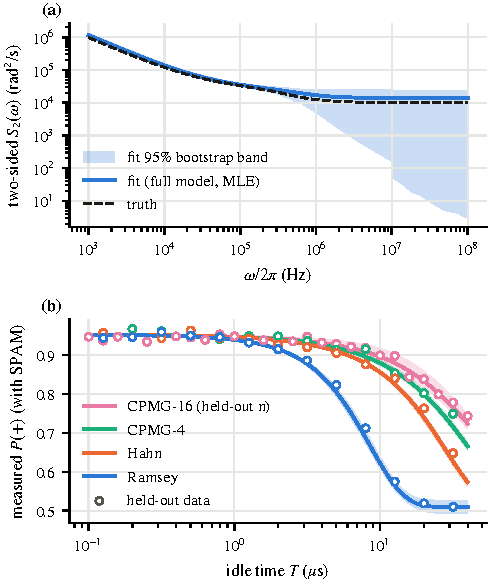
\includegraphics[width=\linewidth]{../figures/fig_spectroscopy.pdf}
\caption{Synthetic spectroscopy. (a) True versus fitted two-sided PSD (full Gaussian model, MLE)
with a 95\% parametric-bootstrap band; above $\sim$1\,MHz the data barely constrain the
spectrum. (b) Fitted decay curves with 95\% bands; open circles are \emph{held-out} data only
(CPMG-16 at all times; other families at unseen times). Run as in Table~\ref{tab:spectroscopy}.}
\label{fig:spec}
\end{figure}

% GENERATED by python scripts/make_report_artifacts.py at commit a49d7bb; do not edit.
\begin{table}[t]
\centering\scriptsize
\caption{Synthetic spectroscopy (gate G4): held-out RMSE of $P(+)$ relative to the shot-noise floor,
95\% predictive coverage on 106 held-out points, and $1/e$ times (fit [95\% bootstrap CI], $\mu$s;
$^\ast$ = CI excludes truth). Truth: $T_2^\ast=9.14\,\mu$s, $T_2^{\rm Hahn}=28.08\,\mu$s.
``telegraph'' = Lorentzian replaced by telegraph noise (misspecification control). Seeds
5001/5002/5003, $n_{\rm boot}=200$. Run \texttt{spectroscopy\_scenario\_a\_20261026T235246Z\_8b272601c344}.}
\label{tab:spectroscopy}
\begin{tabular}{@{}llccccc@{}}\toprule
Truth & Fit model & RMSE/floor & Coverage & $T_2^\ast$ & $T_2^{\rm Hahn}$ & Success\\\midrule
gaussian & full ($\alpha=1$) & 1.15 & 0.934 & 8.40 [7.79, 9.08]$^\ast$ & 26.48 [24.72, 28.00]$^\ast$ & yes \\
gaussian & full ($\alpha$ free) & 1.15 & 0.934 & 8.43 [7.72, 9.04]$^\ast$ & 26.14 [24.63, 28.38] & yes \\
gaussian & reduced & 1.26 & 0.877 & 8.30 [7.71, 8.89]$^\ast$ & 26.52 [25.14, 27.94]$^\ast$ & yes \\
telegraph & full ($\alpha=1$) & 1.05 & 0.962 & 8.69 [8.04, 9.48] & 27.12 [25.28, 29.01] & yes \\
telegraph & reduced & 1.16 & 0.934 & 8.49 [7.86, 9.09]$^\ast$ & 27.29 [25.72, 28.88] & yes \\
\bottomrule\end{tabular}\end{table}


\paragraph{RQ3: CMA-ES versus canonical DD, Scenario~A (pre-registered)}
Table~\ref{tab:bench} and Figs.~\ref{fig:bench} and~\ref{fig:benchratio} report held-out infidelities. The training-only
rule selects XY4 at $n=4$ and XY8 at $n=8,16$, with
$\epsilon=\BenchAFourSelEps$, $\BenchAEightSelEps$ and $\BenchASixteenSelEps$. No CMA-ES mode
gives a practically relevant improvement: the best single run (timing+phase, $n=4$) has ratio
$\BenchAFourBothRatioHi$ with an interval that includes 1, and the other modes are within
$\pm0.2\%$ or worse:
\begin{itemize}
  \item \textbf{Phase-only:} ratios $\BenchASixteenPhaseRatioLo$--$\BenchAFourPhaseRatioHi$
    (\(\approx1\)). The phases it finds are not XY-type: at $n=4$ they form a sign-alternated
    single-axis pattern ($a,\bar a,\bar a,a$), and at $n=8,16$ they are non-canonical. Several
    different phase patterns therefore reach the same floor.
  \item \textbf{Timing+phase:} ratios $\BenchAFourBothRatioLo$--$\BenchAFourBothRatioHi$ at $n=4$
    and at most $\BenchASixteenBothRatioHi$ at $n=8,16$.
  \item \textbf{Timing-only:} ratios as low as $\BenchASixteenTimingRatioLo$. This mode keeps
    CPMG's $Y$ axes, and CPMG with a 2\% amplitude error is far worse than XY4/XY8 under
    gate-fidelity grading (Table~\ref{tab:bench}).
\end{itemize}
The reason there is nothing to gain is physical. XY8 reaches $\BenchASixteenSelEps$, essentially
the pulse-independent floor of $\FloorA$ set by $T_1$ and the white dephasing component
(dashed line in Fig.~\ref{fig:bench}). Under the pre-registered model, no DD sequence can do
much better than XY8. At $T=4\,\mu$s, timing+phase is worse than XY8 (ratio
$\BenchATfourSixteenBothRatioLo$--$\BenchATfourSixteenBothRatioHi$ at $n=16$;
Table~\ref{tab:ablation}).

\begin{figure*}[t]
\centering
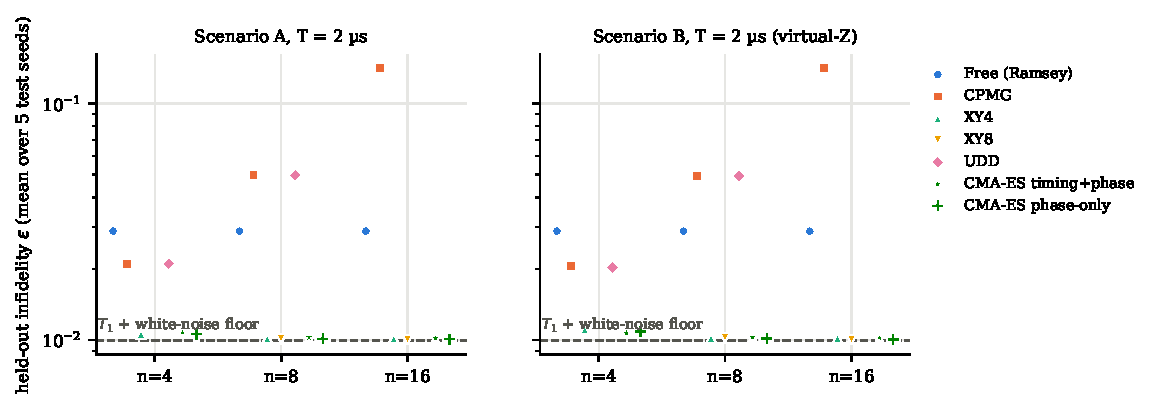
\includegraphics[width=0.92\linewidth]{../figures/fig_benchmark.pdf}
\caption{Held-out infidelity at equal $n$, $T=2\,\mu$s, $w=32$\,ns (mean over test seeds
9001--9005, 1024 trajectories each; CMA-ES: mean over 3 training runs; MC standard errors are
smaller than the markers). The dashed line is the analytic floor from $T_1$ and white noise.
Scenario~B arms use virtual-$Z$ from the nominal Stark profile. Near the floor the markers
overlap; Fig.~\ref{fig:benchratio} shows the comparison with the selected baseline as a ratio.}
\label{fig:bench}
\end{figure*}

\begin{figure}[t]
\centering
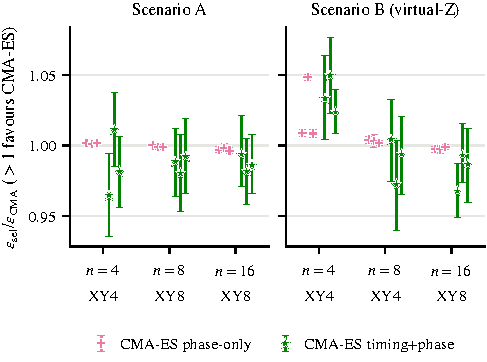
\includegraphics[width=\linewidth]{../figures/fig_benchmark_ratio.pdf}
\caption{Held-out ratio $\epsilon_{\rm sel}/\epsilon_{\rm CMA}$ ($>1$ favours CMA-ES) for each
of the three training runs, with pooled paired-bootstrap 95\% intervals; the training-selected
baseline is named under each $n$. Timing-only CMA-ES (ratios
$\BenchASixteenTimingRatioLo$--$\BenchBFourTimingRatioHi$) is omitted for clarity; see
Table~\ref{tab:bench}.}
\label{fig:benchratio}
\end{figure}

% GENERATED by python scripts/make_report_artifacts.py at commit 995776a; do not edit.
\begin{table*}[t]
\centering\scriptsize\setlength{\tabcolsep}{4pt}
\caption{Held-out benchmark at $T=2\,\mu$s, $w=32$\,ns: infidelity $10^3\epsilon$ averaged over test seeds
9001--9005 (1024 trajectories each; MC standard errors $\lesssim1\%$ of $\epsilon$). ``Sel.'' = baseline
selected by the pre-registered training-only rule. CMA-ES: mean $\epsilon$ over 3 independent training runs and,
in parentheses, the range of $\epsilon_{\rm sel}/\epsilon_{\rm CMA}$ over runs ($>1$ favours CMA-ES).
Scenario~B arms all use virtual-$Z$ from the nominal Stark profile. UDD-16 is infeasible on the grid
(Table~\ref{tab:feasibility}). Runs: \runid{benchmark\_scenario\_a\_20261026T232517Z\_1bd28ade742a}; \runid{benchmark\_scenario\_b\_20261026T234545Z\_ad7b16de1c23}.}
\label{tab:bench}
\begin{tabular}{@{}lc ccccc c ccc@{}}\toprule
 & & \multicolumn{5}{c}{Canonical baselines} & & \multicolumn{3}{c}{CMA-ES (ratio range)}\\
\cmidrule(lr){3-7}\cmidrule(lr){9-11}
Scenario & $n$ & Free & CPMG & XY4 & XY8 & UDD & Sel. & timing-only & phase-only & timing+phase\\\midrule
A & 4 & 28.8 & 20.9 & 10.6 & --- & 21.0 & XY4 & 21.0 (0.500--0.507) & 10.6 (1.001--1.002) & 10.7 (0.965--1.011) \\
 & 8 & 28.8 & 49.7 & 10.2 & 10.1 & 49.8 & XY8 & 49.8 (0.203--0.203) & 10.1 (0.999--1.000) & 10.2 (0.980--0.992) \\
 & 16 & 28.8 & 141.3 & 10.1 & 10.0 & --- & XY8 & 141.4 (0.071--0.071) & 10.1 (0.996--0.998) & 10.2 (0.982--0.994) \\
\addlinespace
B (virtual-$Z$) & 4 & 28.8 & 20.5 & 11.1 & --- & 20.2 & XY4 & 18.6 (0.568--0.612) & 10.8 (1.008--1.048) & 10.7 (1.024--1.050) \\
 & 8 & 28.8 & 49.2 & 10.2 & 10.2 & 49.3 & XY4 & 41.4 (0.245--0.246) & 10.1 (1.002--1.004) & 10.3 (0.972--1.004) \\
 & 16 & 28.8 & 141.1 & 10.1 & 10.0 & --- & XY8 & 109.6 (0.090--0.093) & 10.1 (0.997--0.999) & 10.2 (0.968--0.993) \\
\bottomrule\end{tabular}\end{table*}


\paragraph{Overfitting diagnostic} For a single training run at $n=8$ (exploratory; validation
seeds 8001--8002 are disjoint from the test seeds), the training infidelity of timing+phase
CMA-ES falls to $\ConvTrainFinal$, below XY8's training value. The validation infidelity stays at
$\ConvValFinal$, against $\ConvBestBaselineVal$ for XY8 (Fig.~\ref{fig:conv}). The apparent
training gain comes from fitting the 256 frozen noise trajectories and does not generalize.

\begin{figure}[t]
\centering
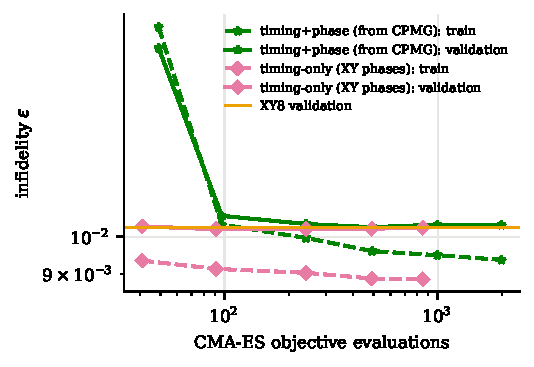
\includegraphics[width=\linewidth]{../figures/fig_convergence.pdf}
\caption{Training (dashed) versus validation (solid) infidelity of the best-so-far CMA-ES
candidate as a function of evaluation budget; Scenario~A, $n=8$, training seed 101.
Timing+phase starts from CPMG; timing-only keeps XY phases. The
horizontal lines show XY8. Exploratory diagnostic.}
\label{fig:conv}
\end{figure}

\paragraph{RQ4: Scenario~B (deterministic Stark-like shift)}
At $n=8$, the four pre-registered arms reach $\epsilon=\BArmNoDD$ (no DD, no frame correction),
$\BArmVzOnly$ (virtual-$Z$ only), $\BArmDDVz$ (best canonical DD + virtual-$Z$) and
$\BArmCMAVz$ (CMA-ES + virtual-$Z$). Most of the benefit comes from frame correction plus any
XY-type DD. At the \emph{nominal} Stark profile, CMA-ES beats XY4+virtual-$Z$ only at $n=4$:
phase-only by ratios $\BenchBFourPhaseRatioLo$--$\BenchBFourPhaseRatioHi$ and timing+phase by
$\BenchBFourBothRatioLo$--$\BenchBFourBothRatioHi$ across the three training runs. The bracket
formed by the three per-run 95\% MC intervals is $\BenchBFourBothCILo$--$\BenchBFourBothCIHi$
for timing+phase. At $n=8,16$ there is no gain (Table~\ref{tab:bench}). These $n=4$ cases were
picked out after inspecting about 27 Scenario~B comparisons, so they are exploratory.

The pre-registered robustness sweep (Table~\ref{tab:robustness}, Fig.~\ref{fig:rob}) changes
the picture for timing+phase. Under $\pm50$--$100$\,ns readout-timing shifts, its worst case
reaches $\RobBFourBothWorstMax$, against $\RobBFourDDWorst$ for XY4+virtual-$Z$, and it wins in
only $\RobBFourBothWinsMin$--$\RobBFourBothWinsMax$ of the 10 perturbed profiles. At $n=8$, two
of three runs lose in all 10. This nominal gain therefore does \emph{not} survive the
uncertainty RQ4 asks about. Only the $n=4$ phase-only sequences remain marginally better than
XY4+virtual-$Z$ in all 10 perturbations in all three runs (worst case
$\RobBFourPhaseWorstMax$ versus $\RobBFourDDWorst$), a few-percent, model-specific effect.
Virtual-$Z$ alone degrades to $\RobBFourVzWorst$ under a $\pm20\%$ amplitude error. Timing
shifts leave it unaffected, because the integrated phase of a shift that stays inside the window
is unchanged.

% GENERATED by python scripts/make_report_artifacts.py at commit eba908c; do not edit.
\begin{table}[t]
\centering\scriptsize\setlength{\tabcolsep}{3pt}
\caption{Scenario~B robustness (pre-registered sweep): worst-case $10^3\epsilon$ over 10 perturbed Stark
profiles (amplitude $\times\{0.8,\dots,1.2\}$, timing $\pm\{50,100\}$\,ns and nominal), virtual-$Z$ always from the
nominal profile; CMA-ES values for training runs 101/102/103, and in how many of the 10 perturbations
CMA-ES beats the selected DD + virtual-$Z$. Run \runid{benchmark\_scenario\_b\_20261026T234545Z\_ad7b16de1c23}.}
\label{tab:robustness}
\resizebox{\columnwidth}{!}{\begin{tabular}{@{}clcccc@{}}\toprule
$n$ & CMA-ES mode & VZ only & DD+VZ & CMA-ES+VZ (runs) & wins/10\\\midrule
4 & phase-only & 38.6 & 11.3 (XY4) & 11.2 / 10.6 / 11.2 & 10 / 10 / 10 \\
4 & timing+phase & 38.6 & 11.3 (XY4) & 16.0 / 14.5 / 21.1 & 8 / 6 / 3 \\
8 & phase-only & 38.6 & 10.2 (XY4) & 10.4 / 10.5 / 10.4 & 8 / 8 / 7 \\
8 & timing+phase & 38.6 & 10.2 (XY4) & 10.7 / 19.9 / 20.8 & 9 / 0 / 0 \\
16 & phase-only & 38.6 & 10.0 (XY8) & 10.4 / 10.1 / 10.2 & 0 / 0 / 0 \\
16 & timing+phase & 38.6 & 10.0 (XY8) & 15.0 / 11.2 / 10.5 & 0 / 0 / 0 \\
\bottomrule\end{tabular}}\end{table}



\begin{figure}[t]
\centering
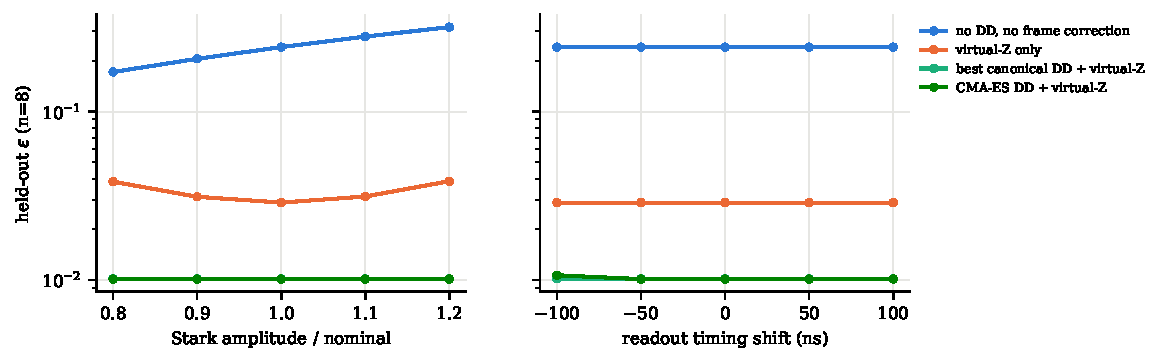
\includegraphics[width=\linewidth]{../figures/fig_robustness_b.pdf}
\caption{Scenario~B robustness at $n=4$, all three training runs: (a) Stark amplitude and
(b) readout timing shift perturbed in evaluation while every virtual-$Z$ angle uses the nominal
profile. Timing+phase CMA-ES (dashed) degrades under timing shifts; phase-only (dotted) does not.}
\label{fig:rob}
\end{figure}

\paragraph{RQ5: robustness, ablations and model mismatch}
Table~\ref{tab:ablation} adds post-hoc ablations, labelled exploratory. Removing $T_1$ and the
white floor (``colored only'') opens two orders of magnitude of headroom, since XY8 then reaches
$\AblColoredSixteenSelEps$ at $n=16$. Even so, timing+phase CMA-ES under the same 2000-evaluation
budget loses to XY8 (ratio $\AblColoredSixteenBothRatioLo$--$\AblColoredSixteenBothRatioHi$),
and phase-only gains at most $\AblColoredFourPhaseRatioHi$ at $n=4$. Within this budget and
parameterization (starting from CPMG, with $2n$ free coordinates), CMA-ES did not find sequences
that generalize better than XY-family designs. The training-only selection rule can itself pick
a baseline that is slightly worse on test (UDD in the no-amplitude-error ablation), which
inflates ratios there by $<1\%$. Robustness to calibration drift, Stark rise time and
timing-grid quantization of the optimized sequences (master-plan item P5.2) was \emph{not} run.
In the model-based pipeline
(Table~\ref{tab:model_based}), optimizing on the noise model \emph{fitted} from synthetic
spectroscopy and testing on the truth gives ratios $\MBFitFullFourRatioLo$--$\MBFitFullFourRatioHi$
(full model, $n=4$) and $\MBFitRedFourRatioLo$--$\MBFitRedFourRatioHi$ (reduced model): model
error adds further loss, and with the reduced model the baseline-selection rule sometimes picks
the weaker family.

% GENERATED by python scripts/make_report_artifacts.py from report/runs.json; do not edit.
\begin{table*}[t]
\centering\scriptsize
\caption{Held-out comparison across scenario variants (test seeds 9001--9005). Ratio
$=\epsilon_{\rm selected}/\epsilon_{\rm CMA}$ (range over 3 training runs; $>1$ favours CMA-ES).
Floor = analytic $T_1$ amplitude damping composed with white dephasing over $T$ (pulse-independent).
$^\dagger$Post-hoc exploratory ablations added after seeing the pre-registered results.}
\label{tab:ablation}
\begin{tabular}{@{}lcccc ccc@{}}\toprule
Variant & $n$ & Sel. & $10^3\epsilon_{\rm sel}$ & $10^3\times$floor & timing-only & phase-only & timing+phase\\\midrule
A (pre-registered), $T=2\,\mu$s & 4 & XY4 & 10.6 & 9.90 & 0.500--0.507 & 1.001--1.002 & 0.965--1.011 \\
 & 8 & XY8 & 10.1 & 9.90 & 0.203--0.203 & 0.999--1.000 & 0.980--0.992 \\
 & 16 & XY8 & 10.0 & 9.90 & 0.071--0.071 & 0.996--0.998 & 0.982--0.994 \\
\addlinespace
A, $T=4\,\mu$s (pre-registered) & 4 & XY4 & 22.8 & 19.6 & 0.693--0.699 & 1.000--1.000 & 0.975--1.003 \\
 & 8 & XY8 & 20.6 & 19.6 & 0.349--0.352 & 0.999--1.000 & 0.939--0.981 \\
 & 16 & XY8 & 19.9 & 19.6 & 0.136--0.136 & 0.997--0.998 & 0.930--0.967 \\
\addlinespace
A without amplitude error$^\dagger$ & 4 & CPMG/UDD & 10.6/10.6 & 9.90 & 0.969--1.007 & 0.999--1.008 & 0.969--1.018 \\
 & 8 & UDD & 10.2 & 9.90 & 0.993--1.007 & 1.007--1.009 & 0.992--1.006 \\
 & 16 & CPMG/XY8 & 10.0/10.0 & 9.90 & 0.987--0.998 & 0.998--0.999 & 0.983--0.997 \\
\addlinespace
A without $T_1$$^\dagger$ & 4 & XY4 & 4.00 & 3.32 & 0.271--0.277 & 1.003--1.004 & 0.917--1.031 \\
 & 8 & XY8 & 3.53 & 3.32 & 0.080--0.081 & 0.996--1.001 & 0.953--1.004 \\
 & 16 & XY8 & 3.45 & 3.32 & 0.025--0.025 & 0.991--0.995 & 0.937--0.994 \\
\addlinespace
A, colored noise only$^\dagger$ & 4 & XY4 & 0.631 & 0.000 & 0.056--0.057 & 1.006--1.010 & 0.967--0.986 \\
 & 8 & XY8 & 0.238 & 0.000 & 0.006--0.006 & 1.002--1.004 & 0.894--0.960 \\
 & 16 & XY8 & 0.098 & 0.000 & 0.001--0.001 & 0.901--0.954 & 0.394--0.566 \\
\bottomrule\end{tabular}\end{table*}

% GENERATED by python scripts/make_report_artifacts.py at commit 9b6b918; do not edit.
\begin{table}[t]
\centering\scriptsize
\caption{Model-based pipeline: baseline selection and CMA-ES (timing+phase) trained on the noise
model in column 1, all arms evaluated on the \emph{true} Scenario~A model (test seeds 9001--9005).
Fitted models come from run \texttt{spectroscopy\_scenario\_a\_20261026T235246Z\_8b272601c344}. Ratio as in Table~\ref{tab:ablation}; CI = envelope of pooled
paired-bootstrap 95\% intervals over the 3 training runs. Run \texttt{model\_based\_scenario\_a\_20261026T235628Z\_373dfea37a30}.}
\label{tab:model_based}
\begin{tabular}{@{}lcccccc@{}}\toprule
Training model & $n$ & Sel. & $\epsilon_{\rm sel}$ & $\epsilon_{\rm CMA}$ & Ratio & CI envelope\\\midrule
true model & 4 & XY4 & $1.06\times10^{-2}$ & $1.07\times10^{-2}$ & 0.965--1.011 & [0.936, 1.037] \\
fitted full model & 4 & XY4 & $1.06\times10^{-2}$ & $1.06\times10^{-2}$ & 0.982--1.011 & [0.960, 1.036] \\
fitted reduced model & 4 & XY4 & $1.06\times10^{-2}$ & $1.11\times10^{-2}$ & 0.894--0.984 & [0.873, 1.005] \\
true model & 8 & XY8 & $1.01\times10^{-2}$ & $1.02\times10^{-2}$ & 0.980--0.992 & [0.952, 1.019] \\
fitted full model & 8 & XY8 & $1.01\times10^{-2}$ & $1.03\times10^{-2}$ & 0.966--0.991 & [0.927, 1.016] \\
fitted reduced model & 8 & XY4/XY8 & $1.01\times10^{-2}$ & $1.07\times10^{-2}$ & 0.896--0.986 & [0.868, 1.011] \\
\bottomrule\end{tabular}\end{table}

% STUB -- NOT GENERATED FROM ANY RUN. Will be overwritten by a script that reads the
% sequence-feasibility results (n, T, pulse width, guard spacing, timing-grid rounding).
\begin{table}[t]
  \centering
  \caption{Timing feasibility of the sequence configurations. \textbf{NOT RUN}: stub table,
    no configurations evaluated.}
  \label{tab:feasibility}
  \begin{tabular}{@{}llllll@{}}
    \toprule
    $n$ & $T$ & Pulse width & Guard & Grid rounding & Feasible \\
    \midrule
    --- & --- & --- & --- & --- & \textbf{NOT RUN} \\
    \bottomrule
  \end{tabular}
\end{table}

